\chapter{Related Work}
\label{chap:relatedwork}
\section{Basics of Genetic Programming}
\subsection{Program Representations}
As is stated in Chapter \ref{chap:intro}, Genetic programming is a general technique that can be applied to almost any task domain.  However, this work predominantly focuses on the task of symbolic regression.  Symbolic regression aims to find a mathematical expression that fits a given data set's training and out of sample test examples.  Therefore the programs in which we are interested define mathematical expressions by combining a set of primitive operations.

Much of the time in genetic programming random segments of code are being removed, inserted, and swapped between different programs.  Therefore, it is important to have a program representation that is resilient to these types of operations.  As a result, it can be useful to avoid loops, and other types of statements that could result in programs that do not terminate.  For this reason, often a tree structure is employed, where the internal nodes of the trees are functions, with the children as the arguments, and the leaves of the trees are terminals, such as variables and constants.

For the task of symbolic regression, the functions can be any set of primitive mathematical functions, while the terminals will typically be the features of the data set.

The tree in Figure \ref{figure:gp_tree} represents a simple program, which computes the mathematical function $f(x) = \ln(x1) + (x1 - x2)$.  Given a larger set of mathematical operations, it is possible to create arbitrarily complex mathematical expressions.

\noindent
\begin{figure}[h]
\centering
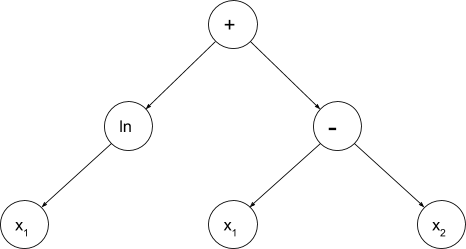
\includegraphics[width=110mm]{gp_tree_colorless}
\caption{Sample tree representing a program.}
\label{figure:gp_tree}
\end{figure}

\subsection{Generating New Programs}
\label{section:gp_operators}
One of the core aspects of genetic programming is how to generate a new population of programs from an old population.  There are two primary operations used to generate new programs: the mutation operation and the crossover operation.

\subsubsection{Mutation}
The mutation operation generates a single new program from a single old program.  First a mutation point is selected in the old program.  This can be selected uniformly at random, or biased towards certain parts of the tree.  Then the subtree located at the mutation point is removed, and a new subtree is generated in a similar way to how the first population of programs was generated.

\subsubsection{Crossover}
The crossover operation generates two new programs from two old programs.  First a crossover point is selected in each old program.  This can be done in any of the same ways that a mutation point is selected.  Then the subtrees located at the two crossover points in the two old programs are swapped, creating two new program trees.

\subsection{Choosing Programs to Survive}
After a new population of programs is generated, only half of the programs from the combined new and old populations are kept for the next generation of the evolutionary process.  If there is a single fitness function that is being optimized, this process is very straightforward.  Simply keep the programs that perform best on the fitness function.  However, often there are multiple fitness functions that are used to drive the evolutionary process.  For example, in the case of symbolic regression, one fitness function could be the absolute error for predicting the dependent variable, while the other fitness function could be the program size.  When there are multiple fitness functions, often one program will have a better fitness score than another program for one fitness function, but not the remaining fitness functions.  In this case a different method must be used to determine which programs should be kept.  The method used for the purpose of this work is discussed in section \ref{section:survival}.

\subsection{Termination}
The run of a genetic program terminates after one of several conditions is met.  The following are common termination conditions:
\begin{enumerate}[noitemsep]
\item An optimal program is found.
\item A maximum number of generations is reached.
\item The run has exceeded the maximum allocated amount of time.
\end{enumerate}

\section{Behavioral Genetic Programming}
One extension to the genetic programming paradigm is behavioral genetic programming (BGP) \cite{krawiec}.  As was mentioned in Chapter \ref{chap:intro}, BGP attempts to identify useful subprograms that can then be used to enhance the evolutionary process.

\subsection{Trace}
In most genetic programming algorithms, the search is driven by the output of the fitness functions alone.  Only programs that perform well on the fitness functions are kept, while the rest are rejected.  However, every subtree that makes up an individual program has a distinct numerical output for each fitness case in any given data set.

Let us consider the program in Figure \ref{figure:gp_tree}, and the sample data set in Table \ref{table:sample_data}.  Conventional genetic programming will only consider the outputs for each data point: $\ln(3) + 1$, $\ln(5) + 2$, and compare those values to the desired output.  However, each subtree has its own output, which is ignored by the genetic programming process.

\begin{table*}[ht]
\centering
\begin{tabular}{ c c | c }
\hline\hline
$x_{1}$ & $x_{2}$ & $y$ \\ [0.5ex]
\hline
3 & 2 & 3 \\
5 & 3 & 4 \\[1ex]
\hline
\end{tabular}
\caption{Sample data set.}
\label{table:sample_data}
\end{table*}

The collection of the outputs on each subtree for all of the data points is called the trace.  For the program in Figure \ref{figure:gp_tree} and the fitness cases in Table \ref{table:sample_data}, the trace is shown in Table \ref{table:sample_trace}.

\begin{table*}[ht]
\centering
\begin{tabular}{ c c c c c c }
\hline\hline
$s_{1}$ & $s_{2}$ & $s_{3}$ & $s_{4}$ & $s_{5}$ & $s_{6}$ \\ [0.5ex]
\hline
3 & $\ln(3)$ & 3 & 2 & 1 & $\ln(3)$ + 1 \\
5 & $\ln(5)$ & 5 & 3 & 2 & $\ln(5)$ + 2 \\[1ex]
\hline
\end{tabular}
\caption{The trace of the program from Figure \ref{figure:gp_tree} for the data set in Table \ref{table:sample_data}.}
\label{table:sample_trace}
\end{table*}

The trace is a matrix where the number of rows is equal to the number of data points, and the number of columns is equal to the number of subtrees in a given program.  There is no set order of the columns, although here they are presented in the depth first traversal order of the subtrees that produce the values.  The trace captures a full snapshot of all of the intermediate states of the program evaluation.

\subsection{Model}
The key idea behind Behavioral Programming is to exploit the trace to identify useful subtrees.  Ordinary crossover does not incorporate any information about the quality of the subtrees that are being swapped.  However, the trace opens up many possibilities to explore the quality of subtrees.  In Behavioral Programming, the trace is used to train a machine learning model to predict the desired output for each fitness case.  The model is then used for two purposes.  The first is to create additional fitness measures by which to evaluate a given program.  The second is to identify useful subtrees based on the composition of this model, which are then placed in an archive.  The content of the archive is then used for the supply the subtrees that are used in the crossover operation, instead of taking arbitrary subtrees from other programs in the population.


